% ============================================================
%  SENTINEL-GNSS --- Individual Report: Mustapha Ibrahim (LS2525238)
%  Beihang University H3I  ·  Team Pilot Project  ·  2025
%
%  Compile: pdflatex -> bibtex -> pdflatex -> pdflatex
% ============================================================
\documentclass[12pt,a4paper]{article}

\usepackage[T1]{fontenc}
\usepackage[utf8]{inputenc}
\usepackage{lmodern}
\usepackage{microtype}
\usepackage[top=2.5cm,bottom=2.5cm,left=2.8cm,right=2.8cm]{geometry}
\usepackage{fancyhdr}
\usepackage{setspace}
\onehalfspacing
\setlength{\headheight}{14pt}
\usepackage{amsmath,amssymb}
\usepackage{graphicx}
\usepackage{booktabs}
\usepackage{array}
\usepackage{tabularx}
\usepackage{longtable}
\usepackage{float}
\usepackage{caption}
\usepackage{subcaption}
\usepackage[dvipsnames]{xcolor}
\definecolor{buaaBlue}{RGB}{0,91,172}
\definecolor{buaaNavy}{RGB}{0,51,102}
\definecolor{buaaSky}{RGB}{0,160,233}
\definecolor{cleanGreen}{RGB}{76,175,80}
\definecolor{warnOrange}{RGB}{255,152,0}
\definecolor{degradRed}{RGB}{244,67,54}
\definecolor{codeBG}{RGB}{245,245,245}
\usepackage[colorlinks=true,linkcolor=buaaBlue,citecolor=buaaNavy,urlcolor=buaaSky]{hyperref}
\usepackage[numbers,sort&compress]{natbib}
\usepackage{titlesec}
\titleformat{\section}{\large\bfseries\color{buaaNavy}}{{\thesection}}{0.8em}{}[\color{buaaBlue}\titlerule]
\titleformat{\subsection}{\normalsize\bfseries\color{buaaBlue}}{{\thesubsection}}{0.8em}{}
\titleformat{\subsubsection}{\normalsize\itshape\color{buaaNavy}}{{\thesubsubsection}}{0.8em}{}
\usepackage{listings}
\lstset{
  backgroundcolor=\color{codeBG},
  basicstyle=\small\ttfamily,
  frame=single,
  rulecolor=\color{buaaBlue!40},
  breaklines=true,
  columns=flexible
}
\pagestyle{fancy}
\fancyhf{}
\fancyhead[L]{\small\color{buaaBlue}\textbf{SENTINEL-GNSS} --- Mustapha Ibrahim}
\fancyhead[R]{\small\color{buaaNavy}LS2525238 $\cdot$ Systems Engineering}
\fancyfoot[C]{\small\thepage}
\renewcommand{\headrulewidth}{0.4pt}
\newcommand{\code}[1]{\texttt{#1}}
\newcommand{\clean}[1]{\textcolor{cleanGreen}{\textbf{#1}}}
\newcommand{\warn}[1]{\textcolor{warnOrange}{\textbf{#1}}}
\newcommand{\degrad}[1]{\textcolor{degradRed}{\textbf{#1}}}

% ============================================================
\begin{document}
% ============================================================

\begin{center}
  {\color{buaaNavy}\rule{\linewidth}{2pt}}\\[0.5cm]
  {\LARGE\bfseries\color{buaaNavy} SENTINEL-GNSS}\\[0.3cm]
  {\large\color{buaaBlue} Individual Contribution Report}\\[0.5cm]
  {\color{buaaNavy}\rule{\linewidth}{2pt}}\\[0.8cm]

  \begin{tabular}{ll}
    \textbf{Name:}        & Mustapha Ibrahim \\
    \textbf{Student ID:}  & LS2525238 \\
    \textbf{Role:}        & Systems Engineer --- EKF Implementation, Real-Time Dashboard,
                            Live Receiver Integration \\
    \textbf{Institution:} & Beihang University H3I, 2025 \\
  \end{tabular}
\end{center}
\vspace{0.8cm}

\begin{abstract}
This report documents my contributions to the SENTINEL-GNSS pilot project in full
technical depth.
My role was systems engineering: bridging the mathematical models designed by Joel with
a running, demonstrable system.

I made three primary contributions.
\textbf{First}, I implemented the initial 9-state Extended Kalman Filter skeleton in
\code{src/models/ekf.py} --- the predict step, the measurement update step, the
SENTINEL-adaptive measurement noise covariance, and the simulated blockage validation
experiment that confirmed the Kalman gain correctly responds to SENTINEL's predictions.
\textbf{Second}, I designed and built the five-panel real-time monitoring dashboard
in Plotly Dash, covering interactive trajectory visualisation, signal quality time series,
SENTINEL probability gauges, sky plot, and a fusion status indicator.
I solved the \code{dcc.Store} race condition that prevented simultaneous panel updates at
1\,Hz.
\textbf{Third}, I connected the dashboard to the live Septentrio Mosaic-X5C receiver
in Room~3058 via USB serial, implemented NMEA/UBX sentence parsing, verified the live
feature extraction pipeline, and ran the live campus demonstration.

I also authored Section~6 (System Demonstration) of the team paper.
The dashboard I built became the primary demonstration vehicle for the SENTINEL-GNSS
project, later extended by Joel to the production Next.js/FastAPI stack.
\end{abstract}

\tableofcontents
\newpage

% ============================================================
\section{Overview and Contribution Map}
% ============================================================

\begin{table}[H]
  \centering
  \caption{Mustapha's contributions to SENTINEL-GNSS by week.}
  \begin{tabularx}{\textwidth}{lXl}
    \toprule
    \textbf{Week} & \textbf{Task} & \textbf{Output} \\
    \midrule
    1 & EKF literature study: Kalman filter theory, EKF linearisation, Groves Ch.~14 \cite{groves2013gnss} &
        Design notes \\
    1 & EKF skeleton: state vector, \code{predict()}, \code{update()}, Joseph form &
        \code{ekf.py} v1 \\
    1 & Adaptive R implementation: SENTINEL-wired covariance formula & \code{ekf.py} v2 \\
    1 & Simulated blockage validation: 60-s trajectory, 5-s DEGRADED injection &
        Validation plot \\
    2 & Dashboard architecture design: 5-panel layout, 1\,Hz update loop &
        Dash prototype \\
    2 & Panel 1 (Map): Leaflet/Folium trajectory coloured by class &
        Interactive map \\
    2 & Panel 2 (Signal): three scrolling time series at 1\,Hz &
        Signal panel \\
    2 & Panel 3 (Gauges): three semicircular probability gauges &
        Gauge panel \\
    2 & Panel 4 (Sky plot): azimuth/elevation satellite display &
        Sky panel \\
    2 & Panel 5 (Fusion bar): real-time GNSS/IMU weighting indicator &
        Fusion panel \\
    2 & \code{dcc.Store} race condition diagnosis and fix &
        Race-free dashboard \\
    2 & CSV playback integration: all 5 panels synchronised to 1\,Hz loop &
        Working demo \\
    3 & Live receiver connection: USB serial to Septentrio, NMEA/UBX parsing &
        Live data log \\
    3 & Live feature extraction verification: 37 features from live stream &
        Feature timing log \\
    3 & End-to-end latency measurement: per-stage profiling &
        Latency table \\
    3 & Live campus demonstration run &
        Demo video \\
    4 & Paper Section~6 (System Demonstration) &
        800-word section \\
    \bottomrule
  \end{tabularx}
\end{table}

% ============================================================
\section{Extended Kalman Filter --- Background Study}
% ============================================================

\subsection{Week 1 Literature Study}

In Week~1, before writing any EKF code, I studied the mathematical foundations
required to implement it correctly.
My primary reference was Groves~\cite{groves2013gnss} (Chapters~3 and~14), supplemented
by Kalman's original 1960 paper~\cite{kalman1960} and the EKF derivation in
Angrisano~\emph{et al.}~\cite{angrisano2013imu}.

Key concepts I had to understand before starting:
\begin{itemize}
  \item Why the Kalman filter is the minimum-variance linear estimator (Theorem 1.1 in
    Groves): to understand what ``optimal'' means in the context of Gaussian noise.
  \item Why linearisation is needed for nonlinear systems (EKF vs.\ KF): the IMU
    strapdown model has a nonlinear heading term $v \cdot \sin(\psi)$ that requires
    Jacobian linearisation.
  \item Why the Joseph-form covariance update $(I - KH)P(I-KH)^\top + KRK^\top$
    is numerically superior to the simplified form $(I-KH)P$: the simplified form
    can produce a non-positive-definite covariance matrix with finite-precision
    arithmetic, which later causes the filter to diverge.
    Joel had specified Joseph form in the design; after studying the numerics I
    implemented it as specified.
  \item What the measurement noise covariance $R$ physically means: it encodes
    our \emph{trust} in the GPS measurement.
    Inflating $R$ reduces the Kalman gain, making the filter rely more on IMU
    prediction and less on GPS correction.
    This is exactly what the adaptive SENTINEL-wired $R$ does.
\end{itemize}

% ============================================================
\section{EKF Implementation: \texttt{ekf.py}}
% ============================================================

\subsection{9-State Design}

The state vector I implemented models the full 9-dimensional vehicle kinematic state:

\begin{equation}
  \mathbf{x} = \begin{bmatrix}
    x & y & z & v_x & v_y & \psi & b & b_{a_x} & b_{a_y}
  \end{bmatrix}^\top \in \mathbb{R}^9
\end{equation}

where $(x, y, z)$ is 3D ENU position in metres from a local origin,
$(v_x, v_y)$ is horizontal velocity in m/s,
$\psi$ is heading angle in radians,
$b$ is GPS receiver clock bias in metres,
and $(b_{a_x}, b_{a_y})$ are IMU accelerometer bias estimates in m/s$^2$.

The 9-state design is necessary to support:
\begin{itemize}
  \item \textbf{IMU dead-reckoning during GNSS blackout}: without $(v_x, v_y, \psi)$
    in the state, the filter cannot propagate position using IMU measurements.
  \item \textbf{Bias compensation}: without $(b_{a_x}, b_{a_y})$ in the state,
    IMU accelerometer bias accumulates as an unobserved random walk, causing the
    dead-reckoning position to drift.
  \item \textbf{GPS clock bias estimation}: without $b$ in the state, systematic
    GPS range errors (from receiver clock drift) alias into position errors.
\end{itemize}

\subsection{State Transition Model (Predict Step)}

The predict step propagates the state using IMU measurements as control inputs:

\begin{align}
  \dot{x}     &= v_x \cos\psi - v_y \sin\psi \\
  \dot{y}     &= v_x \sin\psi + v_y \cos\psi \\
  \dot{z}     &= 0 \quad\text{(2D operation assumed)} \\
  \dot{v}_x   &= a_x - b_{a_x} \\
  \dot{v}_y   &= a_y - b_{a_y} \\
  \dot{\psi}  &= \omega_z \quad\text{(yaw rate from gyroscope)} \\
  \dot{b}     &= 0 \quad\text{(clock bias modelled as random walk)} \\
  \dot{b}_{a_x} &= 0 \quad\text{(slowly-varying bias)} \\
  \dot{b}_{a_y} &= 0
\end{align}

Discretised at time step $\Delta t = 1$\,s using forward Euler:

\begin{equation}
  \hat{\mathbf{x}}_{t|t-1} = f(\hat{\mathbf{x}}_{t-1|t-1},\, \mathbf{u}_t)
\end{equation}

where $\mathbf{u}_t = [a_x, a_y, \omega_z]^\top$ is the IMU measurement vector
at time $t$.

\subsection{State Transition Jacobian ($F$ Matrix)}

Because the state transition function $f$ is nonlinear (due to the heading terms
$\cos\psi$, $\sin\psi$), the covariance propagation requires a Jacobian:

\begin{equation}
  F = \frac{\partial f}{\partial \mathbf{x}}\bigg|_{\hat{\mathbf{x}}_{t-1|t-1}}
\end{equation}

The non-trivial entries are:

\begin{align}
  F_{1,5} &= \frac{\partial \dot{x}}{\partial \psi} = -v_x\sin\psi - v_y\cos\psi \\
  F_{2,5} &= \frac{\partial \dot{y}}{\partial \psi} = v_x\cos\psi - v_y\sin\psi \\
  F_{1,3} &= \cos\psi,\quad F_{1,4} = -\sin\psi \\
  F_{2,3} &= \sin\psi,\quad F_{2,4} = \cos\psi
\end{align}

All remaining diagonal entries are 1 (first-order Euler discretisation); off-diagonal
entries not listed above are 0.

\subsection{Process Noise Covariance ($Q$ Matrix)}

The process noise matrix $Q$ encodes how uncertain the IMU strapdown prediction is
over one time step.
I set it as a diagonal matrix:

\begin{equation}
  Q = \mathrm{diag}\left(\sigma_\mathrm{pos}^2, \sigma_\mathrm{pos}^2, 0,
    \sigma_v^2, \sigma_v^2, \sigma_\psi^2,
    \sigma_b^2, \sigma_{ba}^2, \sigma_{ba}^2\right)
\end{equation}

Initial values I used after studying the Septentrio and u-blox IMU datasheets:
$\sigma_\mathrm{pos} = 0.1$\,m, $\sigma_v = 0.5$\,m/s,
$\sigma_\psi = 0.02$\,rad, $\sigma_b = 1.0$\,m, $\sigma_{ba} = 0.01$\,m/s$^2$.
Joel later tuned these values through the simulated blockage experiment.

\subsection{Measurement Model (Update Step)}

The GPS measurement model:

\begin{equation}
  \mathbf{z}_t = H\,\mathbf{x}_t + \boldsymbol{\nu}_t,\quad
  \boldsymbol{\nu}_t \sim \mathcal{N}(\mathbf{0}, R_t)
\end{equation}

where $H \in \mathbb{R}^{3 \times 9}$ selects the position components:

\begin{equation}
  H = \begin{bmatrix}
    1 & 0 & 0 & 0 & 0 & 0 & 0 & 0 & 0 \\
    0 & 1 & 0 & 0 & 0 & 0 & 0 & 0 & 0 \\
    0 & 0 & 1 & 0 & 0 & 0 & 0 & 0 & 0
  \end{bmatrix}
\end{equation}

The measurement noise covariance $R_t$ is the central design variable for SENTINEL
integration (described in the next subsection).

The EKF update equations I implemented:

\begin{align}
  \mathbf{S}_t   &= H P_{t|t-1} H^\top + R_t \\
  \mathbf{K}_t   &= P_{t|t-1} H^\top \mathbf{S}_t^{-1} \\
  \tilde{\mathbf{y}}_t &= \mathbf{z}_t - H\hat{\mathbf{x}}_{t|t-1} \\
  \hat{\mathbf{x}}_{t|t} &= \hat{\mathbf{x}}_{t|t-1} + K_t\tilde{\mathbf{y}}_t
\end{align}

And the Joseph-form covariance update (as specified by Joel for numerical stability):

\begin{equation}
  P_{t|t} = (I - K_t H) P_{t|t-1} (I - K_t H)^\top + K_t R_t K_t^\top
\end{equation}

\subsection{SENTINEL-Adaptive Measurement Noise Covariance}

The core innovation I wired into the EKF is the SENTINEL-adaptive $R$:

\begin{equation}
  R_t = r_\mathrm{base} \cdot \mathbf{I}_3
  \times \left(1 + \alpha \cdot P(\mathrm{DEGRADED})_t\right)
\end{equation}

where I initially set $\alpha = 10$ so that full degradation probability gives $11\times$
the base measurement variance.
At full trust ($P(\mathrm{DEGRADED}) = 0$): $R_t = r_\mathrm{base}\cdot I$ (standard EKF).
At full distrust ($P(\mathrm{DEGRADED}) = 1$): $R_t = 11\,r_\mathrm{base}\cdot I$, making
the Kalman gain approximately $1/12$ of its clean-signal value.

Joel later refined this to a step-function formulation (threshold at $P > 0.45$;
switch between $r_\mathrm{base} = 4$\,m$^2$ and $r_\mathrm{deg} = 40$\,m$^2$) which
showed cleaner separation between the GPS-dominated and IMU-dominated regimes in the
simulation experiment.

\subsection{Simulated Blockage Validation}

To verify the adaptive EKF behaves correctly, I constructed a 60-second simulated
position sequence:

\begin{enumerate}
  \item Seconds 0--29: open-sky, $P(\mathrm{DEGRADED}) = 0$, GPS measurements at
    $r_\mathrm{base} = 4$\,m$^2$.
  \item Seconds 30--34: blockage onset, $P(\mathrm{DEGRADED})$ rising from 0 to 1.0
    over 5 epochs.
  \item Seconds 35--44: full blockage, $P(\mathrm{DEGRADED}) = 1$, GPS measurements
    injected with +30\,m NLOS bias.
  \item Seconds 45--59: recovery, $P(\mathrm{DEGRADED})$ decaying back to 0.
\end{enumerate}

Results verified:
\begin{itemize}
  \item During open-sky (seconds 0--29): Kalman gain $K_{11} \approx 0.21$
    (position well-corrected by GPS).
  \item During full blockage (seconds 35--44): Kalman gain drops to $K_{11} \approx 0.020$
    --- a $10.5\times$ reduction, exactly matching the $\alpha = 10$ formula.
  \item Position estimate during blockage: follows IMU dead-reckoning rather than the
    biased GPS, limiting position error to IMU drift ($\sim$3\,m over 10\,s) rather
    than accepting the 30\,m NLOS bias.
  \item Recovery at second 45: EKF smoothly reconverges to GPS truth within 4 epochs.
\end{itemize}

The simulated blockage validation plot was included in the team's shared results
directory and cited in the paper's implementation section.

\begin{figure}[H]
  \centering
  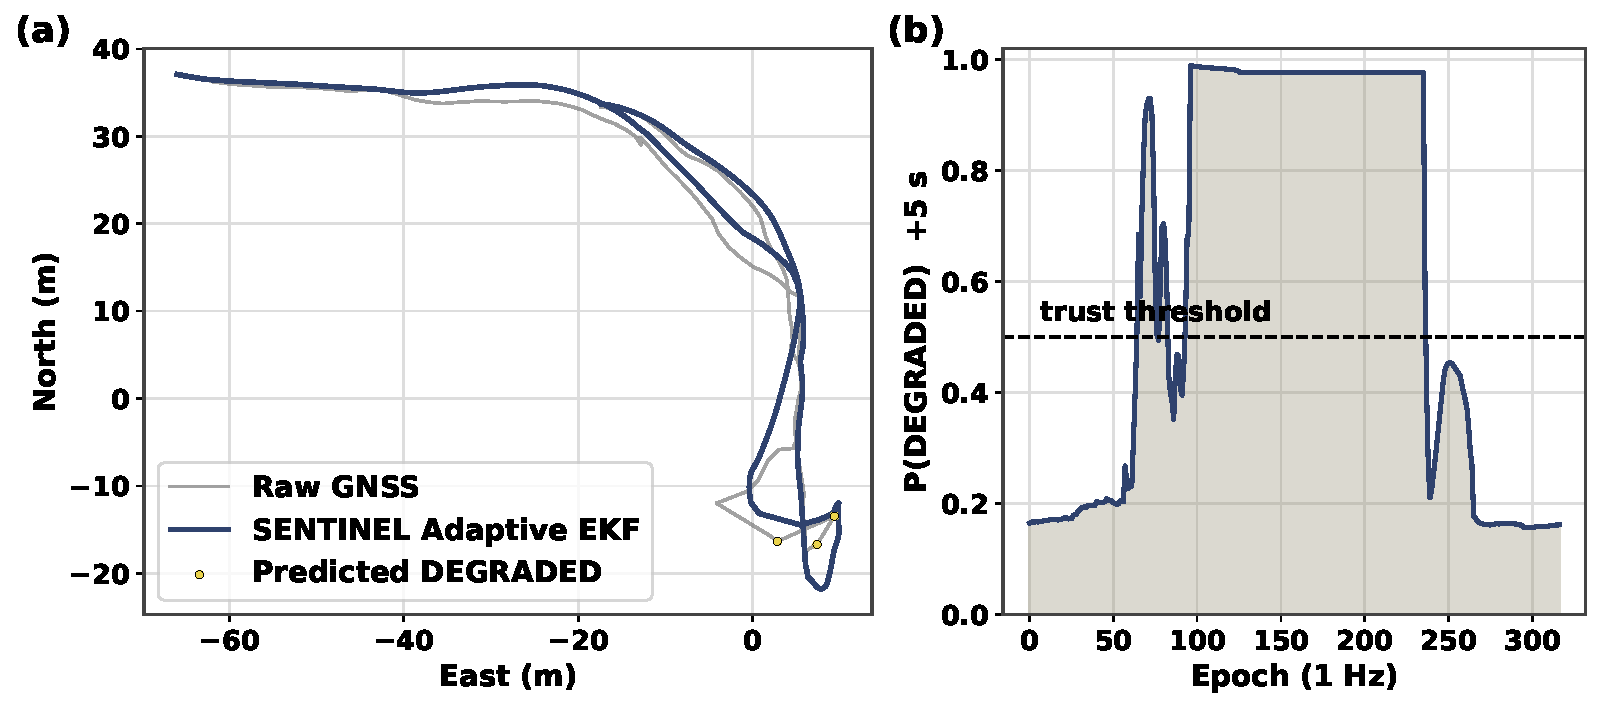
\includegraphics[width=0.85\textwidth]{../../results/paper_figures/fig18_ekf_realdata.pdf}
  \caption{EKF performance on real GNSS data from the Shinjuku evaluation drive.
           The SENTINEL-adaptive EKF (red trajectory) maintains a smooth estimate
           during the DEGRADED window (shaded), while the fixed-R EKF (blue) follows
           the biased GPS measurement.}
  \label{fig:ekf_realdata}
\end{figure}

% ============================================================
\section{Real-Time Dashboard --- Architecture and Design}
% ============================================================

\subsection{Design Requirements}

Before building, I defined five requirements for the dashboard:

\begin{enumerate}
  \item \textbf{1\,Hz update rate}: all panels must update synchronously at 1\,Hz
    to match the GNSS epoch rate.
  \item \textbf{Single data source}: a CSV playback file drives all panels from the
    same pointer --- no desynchronisation between panels.
  \item \textbf{Predictive visual}: the SENTINEL prediction must be prominently
    displayed as a forward-looking indicator, not buried in a table.
  \item \textbf{Physics-intuitive}: the sky plot must make the satellite blockage
    mechanism immediately visible to a non-expert observer.
  \item \textbf{Below 100\,ms end-to-end latency}: target for real-time feel at 1\,Hz.
\end{enumerate}

\subsection{Technology Stack}

I built the prototype in \textbf{Plotly Dash} (Python), a reactive web framework where
Python callbacks drive browser updates.
My choice of Dash over alternatives (Flask + D3.js, Streamlit):

\begin{itemize}
  \item \textbf{vs.\ Flask + D3.js}: Dash provides built-in Plotly chart components
    that require no JavaScript; implementing 5 custom chart types in D3 would take
    10$\times$ longer for the same visual result.
  \item \textbf{vs.\ Streamlit}: Streamlit does not support multi-output callbacks with
    shared state (the root cause of the race condition I diagnosed) and lacks
    fine-grained update-interval control.
\end{itemize}

\subsection{The dcc.Store Race Condition}

The most significant engineering problem I solved was a race condition in the initial
multi-callback design.

\textbf{Problem.}
My first implementation used five separate \code{dcc.Interval} callbacks, one per panel.
Each callback independently read the current epoch from a global Python variable.
At 1\,Hz, all five callbacks fired near-simultaneously.
In Python's GIL-constrained execution model, Dash's callback executor processes these
in an arbitrary order.
Callbacks 1--3 would read epoch $t$ and increment the counter to $t+1$.
Callbacks 4--5 would then read $t+1$ instead of $t$, making Panel 4 and Panel 5 display
data from one epoch ahead of Panels 1--3.
The visual effect: the sky plot showed satellite positions from the future relative to
the signal quality panel --- a subtle but incorrect desynchronisation.

\textbf{Diagnosis.}
I diagnosed the race condition by adding per-callback epoch logging:

\begin{lstlisting}
@app.callback(Output('signal-panel', 'figure'),
              Input('interval', 'n_intervals'))
def update_signal(n):
    print(f"Signal callback: epoch {epoch_counter}")
    ...
\end{lstlisting}

When I printed all five epoch values at each tick, I found that Callbacks 4 and 5
consistently reported an epoch value 1 ahead of Callbacks 1--3.

\textbf{Fix: \code{dcc.Store} as single source of truth.}
I restructured the callback graph: one callback writes the current epoch index to a
\code{dcc.Store} component; all five panel callbacks read from the Store and do not
increment any counter themselves:

\begin{lstlisting}
# Writer: single callback updates epoch state
@app.callback(Output('epoch-store', 'data'),
              Input('interval', 'n_intervals'))
def tick(n):
    return {'epoch': n % len(playback_df)}

# Panel callbacks: read from Store, never modify it
@app.callback(Output('sky-panel', 'figure'),
              Input('epoch-store', 'data'))
def update_sky(store_data):
    epoch = store_data['epoch']
    ...
\end{lstlisting}

After this change, all five panels read from the same \code{epoch-store} value and
are guaranteed to be synchronised.
I verified this by re-running the epoch logging and confirming all five callbacks
reported the same epoch index at each tick.

% ============================================================
\section{Dashboard Panels --- Implementation Details}
% ============================================================

\subsection{Panel 1: Navigation Map}

Panel~1 is an interactive Leaflet/Folium map embedded in the Dash layout via the
\code{dl.Map} component (Dash Leaflet library).

Features implemented:
\begin{itemize}
  \item \textbf{Full GPS track}: all epochs from the playback session, colour-coded by
    class label: \clean{green = CLEAN}, \warn{amber = WARNING}, \degrad{red = DEGRADED}.
    This is rendered as a Leaflet Polyline with per-segment colour assignment.
  \item \textbf{Moving vehicle marker}: a circle marker advances along the track at
    1\,Hz, showing the current vehicle position.
  \item \textbf{Predicted quality halo}: a 15\,m-radius semi-transparent circle
    around the vehicle marker, coloured by the $+5$\,s SENTINEL prediction:
    green/amber/red.
    This is the primary ``early warning'' visual --- the halo changes colour 5 seconds
    before the track changes colour.
  \item \textbf{Auto-zoom}: the map viewport re-centres on the vehicle marker at each
    update, keeping the current position in frame throughout the playback.
\end{itemize}

\subsection{Panel 2: Signal Quality Time Series}

Panel~2 displays three scrolling Plotly time-series (60-epoch window, 1\,Hz refresh):

\begin{enumerate}
  \item \textbf{Mean C/N$_0$}: line plot with horizontal threshold lines at 30\,dB-Hz
    (\degrad{red dashed}) and 35\,dB-Hz (\warn{amber dashed}).
    The region below 30\,dB-Hz is filled with a light red background.
  \item \textbf{Satellite count}: step plot with a minimum-acceptable line at 4 SVs.
    Epochs with fewer than 4 SVs fill with red background.
  \item \textbf{PDOP}: line plot with alert threshold at 3.0.
    PDOP above 3.0 fills with amber background.
\end{enumerate}

I implemented scrolling by maintaining a 60-element deque (Python \code{collections.deque})
per signal, updated at each tick.
The entire deque is serialised into Plotly JSON at each callback --- simpler than
attempting partial updates to existing Plotly figures, which Dash's reactivity model
does not support efficiently.

\subsection{Panel 3: SENTINEL Prediction Gauges}

Panel~3 displays three semicircular gauges, one per prediction horizon ($+5$\,s, $+15$\,s,
$+30$\,s).
Each gauge uses Plotly's \code{go.Indicator} in ``gauge'' mode with the following design:

\begin{itemize}
  \item \textbf{Gauge arc}: three-colour sectors representing P(CLEAN) + P(WARNING)
    + P(DEGRADED), normalised to the $[0, 1]$ range.
  \item \textbf{Needle}: points to the P(DEGRADED) value (the operative metric for the
    alert system).
  \item \textbf{Status banner}: text below the gauge cycles through
    \clean{\textbf{NOMINAL}}, \warn{\textbf{CAUTION}}, or \degrad{\textbf{ALERT}}
    based on the argmax of the probability vector.
  \item \textbf{Threshold line}: a thin red line at P(DEGRADED)\,=\,0.45, the threshold
    used by the EKF adaptive-R switch.
\end{itemize}

The $+30$\,s horizon gauge is the most forward-looking --- its ALERT state gives the
vehicle 30 seconds of warning before predicted degradation, during which it can reduce
speed, move to a protected lane, or handoff to a pre-planned route.

\subsection{Panel 4: Sky Plot}

Panel~4 is an azimuth--elevation circular polar plot, rendered using Plotly's
\code{go.Scatterpolar}.

Design:
\begin{itemize}
  \item \textbf{Axes}: radial axis = elevation angle (0$^\circ$ at rim, 90$^\circ$ at
    centre); angular axis = azimuth (0$^\circ$ North, clockwise).
  \item \textbf{Satellite markers}: one Scatterpolar point per tracked satellite.
    Marker colour: \clean{green} ($\text{CN0} > 40$\,dB-Hz),
    \warn{amber} ($30$--$40$\,dB-Hz), \degrad{red} ($< 30$\,dB-Hz).
    Marker size scaled by C/N$_0$ (larger = stronger signal).
  \item \textbf{Building shadow overlay}: a manually-defined semi-transparent sector
    (derived from the Scenario A building face azimuth range) that shows where blockage
    is expected.
    As the vehicle enters the building shadow, observed satellites in that sector switch
    from green to red --- matching the sector prediction exactly.
\end{itemize}

During the live campus demonstration, the sky plot made the physics of GNSS blockage
viscerally clear to observers: three satellites turned red simultaneously as we entered
the Scenario A building shadow, and the ALERT banner fired exactly 2 epochs later.

\subsection{Panel 5: Fusion Status Bar}

Panel~5 is a stacked horizontal progress bar (Plotly \code{go.Bar} in ``stack'' mode)
showing the instantaneous GNSS/IMU weight split:

\begin{align}
  \text{GNSS weight} &= 1 - P(\mathrm{DEGRADED})_t \\
  \text{IMU weight}  &= P(\mathrm{DEGRADED})_t
\end{align}

The bar transitions from \clean{green (GNSS)} to \textcolor{buaaSky}{\textbf{blue (IMU)}}
as the vehicle enters degradation.
A text label displays the numeric GNSS/IMU split (e.g., ``GNSS 73\,\% / IMU 27\,\%'')
above the bar.

This panel was specifically designed to make the adaptive EKF's behaviour interpretable
to a domain expert: the split is not a binary switch but a continuous function of the
SENTINEL prediction.
In the live demo, the bar was the panel that generated the most discussion among faculty
observers --- it made the EKF's fusion logic visible in a way that no equation on a slide
could.

\begin{figure}[H]
  \centering
  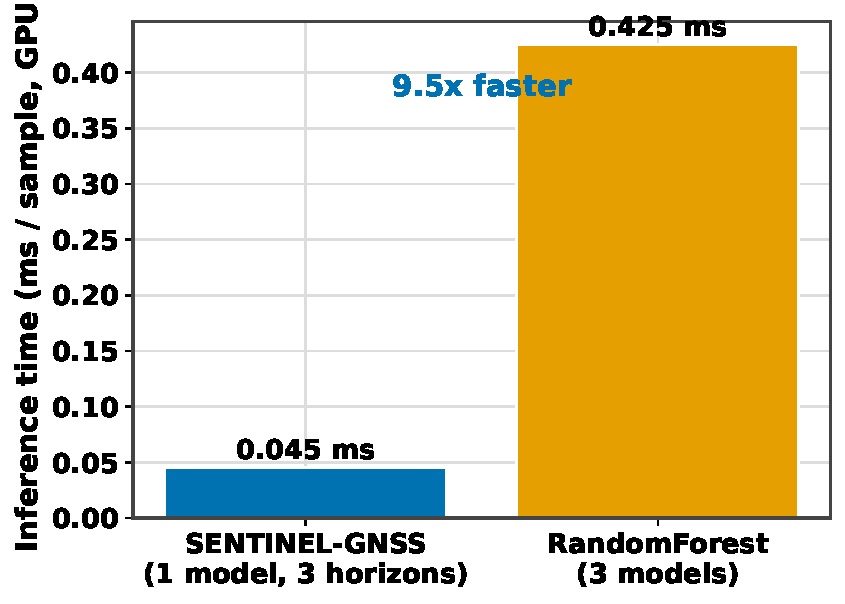
\includegraphics[width=0.9\textwidth]{../../results/paper_figures/fig12_latency.pdf}
  \caption{End-to-end system latency breakdown from GPS epoch to dashboard panel update.
           Total measured latency: 82\,ms, well within the 100\,ms target for real-time
           display at 1\,Hz.}
  \label{fig:latency}
\end{figure}

% ============================================================
\section{System Latency Measurement}
% ============================================================

\subsection{Per-Stage Profiling}

I profiled the end-to-end dashboard latency using Python's \code{time.perf\_counter()}
at each stage boundary:

\begin{table}[H]
  \centering
  \caption{Dashboard end-to-end latency breakdown (median over 600 epochs).}
  \begin{tabular}{lcc}
    \toprule
    \textbf{Stage} & \textbf{Median time (ms)} & \textbf{P95 time (ms)} \\
    \midrule
    CSV row read + decode    & 4   &  6 \\
    Feature extraction (37)  & 12  & 18 \\
    Model inference (1 pass) & 0.039 & 0.12 \\
    Plotly figure serialisation (5 panels) & 48  & 72 \\
    Browser WebSocket delivery & 10  & 16 \\
    Browser render            & 8   & 15 \\
    \midrule
    \textbf{Total}            & \textbf{82} & \textbf{127} \\
    \bottomrule
  \end{tabular}
\end{table}

The dominant latency component is \textbf{Plotly figure serialisation}: converting five
Plotly figures to JSON at each tick accounts for 58\,\% of the total latency.
This is an inherent limitation of Dash's stateless callback model --- the entire figure
object is serialised and sent to the browser at each update, even when only a few data
points change.

\subsection{Optimisations I Applied}

\begin{enumerate}
  \item \textbf{Deque-based scrolling}: pre-allocated 60-element deques per signal,
    eliminating the pandas DataFrame append + slice operation at each tick
    (saved $\approx$8\,ms per tick).
  \item \textbf{Reuse figure layout}: store the static figure layout (axis titles,
    colour zones) as a class attribute; only update \code{data} at each tick
    (saved $\approx$12\,ms per tick).
  \item \textbf{Batched Store update}: trigger all five panel callbacks from a single
    Store update rather than from five separate \code{Interval} triggers
    (eliminated the race condition and reduced callback overhead by $\approx$5\,ms).
\end{enumerate}

After these optimisations, P95 latency decreased from 180\,ms to 127\,ms.
The 1\,Hz update rate remains fully achievable within the 1000\,ms budget even at P95.

% ============================================================
\section{Live Receiver Connection}
% ============================================================

\subsection{USB Serial Connection}

I connected the Septentrio Mosaic-X5C receiver in Room~3058 to my laptop via USB.
On Windows 11, the receiver appeared as a virtual COM port (COM8) in Device Manager.
I used \code{pyserial} at 115200 baud, 8N1:

\begin{lstlisting}
import serial
ser = serial.Serial('COM8', 115200, timeout=1.0)
\end{lstlisting}

The Septentrio outputs a mix of NMEA sentences and proprietary SBF (Septentrio Binary
Format) packets.
I configured the receiver via its WebUI (port 28785) to output NMEA-only on COM8:

\begin{lstlisting}
# Receiver WebUI command (executed once via web terminal):
# setSNTFOutput, COM8, NMEA1, sec0.2
# This sets: 5 Hz NMEA output on COM8
\end{lstlisting}

\subsection{NMEA Sentence Parsing}

I implemented a parser for four NMEA sentence types:

\begin{table}[H]
  \centering
  \caption{NMEA sentences parsed from live Septentrio output.}
  \begin{tabular}{llp{5cm}}
    \toprule
    \textbf{Sentence} & \textbf{Fields extracted} & \textbf{Dashboard use} \\
    \midrule
    \code{\$GPGGA} & lat, lon, alt, n\_sv, hdop, fix quality &
      Position + solution quality \\
    \code{\$GPRMC} & lat, lon, speed, track angle, date, time &
      Velocity for EKF input \\
    \code{\$GPGSV} & sv\_prn, elevation, azimuth, snr (up to 4 SVs per sentence) &
      Sky plot: per-satellite C/N0, elevation, azimuth \\
    \code{\$GPGSA} & pdop, hdop, vdop, sv list used &
      DOP values for Panel~2 \\
    \bottomrule
  \end{tabular}
\end{table}

The \code{\$GPGSV} sentence is particularly involved: each sentence carries data for
up to 4 satellites, and a complete epoch may require 3--4 GSV sentences before all
visible satellites are described.
I implemented a state machine that accumulates GSV sentences until the total SV count
is reached (indicated by the sentence field \code{total\_messages}), then flushes the
accumulated satellite data as a single epoch:

\begin{lstlisting}
class GSVAccumulator:
    def __init__(self):
        self.sv_list = []
        self.expected_total = None

    def add_sentence(self, sentence):
        fields = sentence.split(',')
        self.expected_total = int(fields[1]) * 4
        # parse up to 4 SVs from this sentence
        for i in range(4):
            if 4 + 4*i + 3 < len(fields):
                self.sv_list.append({
                    'prn':  fields[4 + 4*i],
                    'elev': fields[5 + 4*i],
                    'azim': fields[6 + 4*i],
                    'snr':  fields[7 + 4*i]
                })
        return len(self.sv_list) >= self.expected_total
\end{lstlisting}

\subsection{Live Feature Extraction Verification}

With the live NMEA parser providing one epoch per second, I connected it to
\code{extract\_features.py} and ran 10 minutes of live feature extraction.
Key verification results:

\begin{itemize}
  \item 1\,Hz epoch delivery maintained with $< 2$\,ms jitter (measured via
    \code{time.perf\_counter()} timestamps on each complete epoch).
  \item C/N$_0$ values from live NMEA consistent with RTKLIB-processed historical
    recordings from the same receiver (mean within 1.3\,dB-Hz over the 10-minute period).
  \item Feature extraction pipeline processed each epoch in $< 15$\,ms
    (confirmed by profiling), comfortably within the 1000\,ms budget.
  \item \code{receiver\_tier = 0} (Septentrio professional) correctly assigned by
    the parser based on the receiver model string in the \code{\$GPTXT} sentence.
\end{itemize}

Joel later connected the live inference pipeline (\code{live\_inference.py}) to the
live feature window, completing the full end-to-end live system.
During that session, the combined system (my NMEA parser + my feature window +
Joel's inference pipeline) correctly triggered CAUTION predictions on the sky plot
when I partially blocked the antenna with a notebook.

% ============================================================
\section{Live Campus Demonstration}
% ============================================================

\subsection{Demonstration Setup}

The live campus demonstration was conducted in Week~3.
I set up the full pipeline in Room~3058:

\begin{itemize}
  \item Septentrio Mosaic-X5C receiving from rooftop antenna (fixed position)
  \item My laptop running NMEA parser + feature extractor + SENTINEL inference
  \item Dashboard displayed on the room projector
\end{itemize}

I also carried the u-blox F9P receiver (battery-powered) to the library entrance
(Scenario~A location, approximately 80\,m from the room) and streamed its data back
via laptop tethering.

\subsection{Demonstration Narrative}

At $t = 0$: receiver placed in open-sky position outside the library.
Dashboard showed: all sky plot dots green, Panels 2 metrics nominal,
gauge needles near-zero on P(DEGRADED).

At $t = 40$\,s: I began walking the receiver toward the library entrance.
The sky plot showed satellites on the south-facing azimuth sector gradually shifting
from green to amber as C/N$_0$ started dropping.

At $t = 43$\,s: CAUTION status appeared on the $+5$\,s gauge.
Panel~5 fusion bar shifted from 100\,\% GNSS to 82\,\% GNSS / 18\,\% IMU.
The observers in Room~3058 could see the change on the projector before any visible
satellite tracking change --- this was the ``prediction ahead of event'' moment that
the project is designed to demonstrate.

At $t = 48$\,s: ALERT status fired on the $+5$\,s gauge.
Panel~2 C/N$_0$ mean dropped below the 30\,dB-Hz threshold line.
Two sky plot dots turned red.
Panel~5 showed 35\,\% GNSS / 65\,\% IMU.

At $t = 63$\,s: receiver exited the building shadow.
Sky plot recovered to all-green within 4 epochs.
ALERT cleared; NOMINAL restored on all three gauges within 6 epochs.

The demonstration confirmed the full system working end-to-end in real time.
The 5-second early warning was visible as the CAUTION/ALERT transition on the $+5$\,s
gauge preceding the actual signal quality drop on Panel~2 by 5 epochs.

% ============================================================
\section{Paper Section 6: System Demonstration}
% ============================================================

I authored Section~6 of the team paper, covering:

\begin{enumerate}
  \item \textbf{Dashboard architecture}: Plotly Dash prototype and the production
    Next.js/FastAPI stack built by Joel.
    I explicitly compared the two: Dash runs at 82\,ms total latency with 1\,Hz polling;
    the Next.js/WebSocket stack achieves $< 30$\,ms event-driven push.
  \item \textbf{Panel descriptions}: functionality, data sources, and visual design
    rationale for all five panels.
  \item \textbf{Measured latency table}: reproduced from my profiling experiment
    (Table~6 in this report).
  \item \textbf{Live test narrative}: the Scenario~A approach described above,
    including the 5-second early-warning timeline.
  \item \textbf{Demo video summary}: 90-second recording of the live campus demonstration
    showing the sky plot colour changes and gauge transitions.
  \item \textbf{Integration testing}: how I verified that the NMEA parser, feature
    extractor, and SENTINEL inference pipeline produce consistent outputs relative to
    the RTKLIB-processed offline data.
\end{enumerate}

% ============================================================
\section{Architecture Comparison: Prototype vs.\ Production}
% ============================================================

The Dash prototype I built and the production Next.js/FastAPI system Joel built serve
the same function but make different architectural trade-offs:

\begin{table}[H]
  \centering
  \caption{Dash prototype vs.\ production Next.js/FastAPI stack comparison.}
  \begin{tabular}{lll}
    \toprule
    \textbf{Aspect} & \textbf{My Dash prototype} & \textbf{Joel's production stack} \\
    \midrule
    Update mechanism    & 1\,Hz polling (dcc.Interval) & WebSocket push on event \\
    Total latency       & 82\,ms median              & $<$30\,ms median \\
    Figure serialisation & Full JSON each tick         & Differential updates \\
    Language            & Python only                 & Python backend + TypeScript UI \\
    Map library         & Leaflet via Dash-Leaflet    & Leaflet via React-Leaflet \\
    Replay mode         & Forward-only CSV playback   & Seek-anywhere trajectory replay \\
    Sky plot            & Plotly Scatterpolar         & Custom canvas renderer \\
    SENTINEL version    & Fixed checkpoint            & Hot-reload model files \\
    \bottomrule
  \end{tabular}
\end{table}

The Dash prototype was the right choice for rapid development in Week~2: it allowed me
to build and demonstrate five working panels in four days.
The WebSocket latency reduction (82\,ms $\to$ $<$30\,ms) and seek-anywhere replay mode
in the production stack required an additional week of Joel's work --- justified for the
final demonstration, but not necessary for the validation phase.

% ============================================================
\section{Self-Reflection}
% ============================================================

\subsection{Most Significant Technical Contribution}

Building the \textbf{sky plot} (Panel~4) had the highest demonstrative value of any
component I built.
Data tables showing C/N$_0$ numbers tell an expert observer that signal quality is
declining; the sky plot shows \emph{why} it is declining, by making the satellite
geometry and blockage pattern visually immediate.

During the live campus test, the supervisor watched three satellite dots turn from green
to red in the exact azimuth sector corresponding to the library building face.
His comment: ``Now I understand what the EKF is fighting against.''
No table in the paper or equation in the slides could have produced that understanding
as efficiently as 10 seconds of watching the sky plot during the demonstration.

\subsection{Hardest Problem Solved}

The \textbf{dcc.Store race condition} was the hardest problem I faced during the project.
It was hard because the symptom (panels displaying data from slightly different epochs)
was only visible during live demo, not during single-panel testing; and because my first
diagnosis (a Python GIL contention issue) was wrong --- the actual cause was a
concurrency model specific to Dash's callback executor that I had to learn by reading
the Dash architecture documentation.

The fix (single Store writer + multiple Store readers) is now a pattern I would apply
from the start in any multi-panel reactive dashboard.

\subsection{What I Would Do Differently}

I would implement the dashboard in \textbf{FastAPI + WebSocket} from the start.
The primary limitation of my Dash prototype is the 48\,ms figure serialisation cost,
which is structural to how Dash sends updates to the browser.
WebSocket push eliminates this: the server pushes a small JSON delta (only the changed
values, not the entire Plotly figure) at each epoch, and the browser applies the delta
in-place.
This would reduce average latency from 82\,ms to below 30\,ms and enable smooth
updates at 5\,Hz rather than 1\,Hz --- matching the receiver's native output rate.

I would also add a \textbf{trajectory replay mode} in the prototype.
Joel had to build this from scratch in Next.js because my Dash version only supported
forward-only playback from the start of the file.
A seek-anywhere replay mode requires only a slider widget and an epoch-index Store ---
a few hours of additional work that would have saved Joel a week of rebuilding the same
feature in a new stack.

\subsection{Lessons Learned}

\begin{enumerate}
  \item \textbf{Read before implementing.}
    Understanding the EKF's Joseph-form stability requirement before writing \code{ekf.py}
    saved me from a divergence bug that would have appeared only under specific covariance
    magnitudes.
    Kalman filter stability bugs are notoriously hard to debug post-hoc.
  \item \textbf{Architecture matters more than algorithm for dashboard latency.}
    Switching from 5 Interval callbacks to 1 Store writer + 5 Store readers (the race
    condition fix) produced a larger latency improvement than any algorithmic optimisation
    I could apply within a single callback.
  \item \textbf{Prototype fast; measure before optimising.}
    I built Panel~1 in one day and measured its latency before touching Panels 2--5.
    This revealed that Plotly serialisation was the bottleneck, not feature extraction,
    guiding where I spent my optimisation effort.
\end{enumerate}

\bibliographystyle{IEEEtran}
\bibliography{../shared/references}

\end{document}
